\begin{framed}

Objetivos:
\begin{itemize}
    \item Estudiar las propiedades de la ecuación de Laplace. 
    \item Presentar flujos potenciales elementales. 
\end{itemize}

Contenidos:
\begin{itemize}
    \item Repaso de flujos ideales.
    \item Propiedades de la ecuación de Laplace.
    \item Flujos potenciales elementales.
    \item Ejemplos de aplicación de flujos potenciales.
\end{itemize}

Bibliografía:
\begin{itemize}
    \item White, F. M. (2008) Mecánica de Fluidos. McGraw-Hill. Sexta edición. Secciones 4.9-4.10
    \item Fox, R. W., Pritchard, P. J. y McDonald, A. T. (2009) Introduction to Fluid Mechanics. John Wiley \& Sons. Sección 6.7.
\end{itemize}
\end{framed}

\section*{Flujo potencial}
La clase pasada introducimos un par de conceptos nuevos, al menos en el contexto de mecánica de fluidos: la función corriente ($\psi$) y la función potencial ($\phi$). 
Un campo de velocidad tiene una función corriente cuando éste tiene divergencia nula y bidimensional, y tiene una función potencial cuando es irrotacional, donde
%
\begin{align}\label{eq:phi_def_3}
u &= \frac{\partial\phi}{\partial x} = \frac{\partial\psi}{\partial y}\nonumber\\
v &= \frac{\partial\phi}{\partial y} = -\frac{\partial\psi}{\partial x}
\end{align}
%
Físicamente, esto significa que el flujo debe ser incompresible y no viscoso, o sea, un \emph{flujo ideal}.

En la vida real, no exiten los flujos totalmente ideales, pero hay ciertas situaciones en que se comportan muy cercano a ideal y la teoría de flujo potencial nos ayuda a modelarlos.
Dos ejemplos son
\begin{itemize}
\item Flujo sobre cuerpos sumergidos, lejos de cuerpo: muy aplicado a aerodinámica, que revisaremos en un par de clases más. El flujo se ve afectado cerca del cuerpo, pero si uno se aleja de este, el flujo es prácticamente potencial.
\item Tornados: el flujo atmosférico de escala ``global'' puede ser visto como bidimiensional, ya que la dimensión de altura es muchísimo más chica que la extensión en los otros sentidos. Un tornado se aproxima muy bien por un vórtice ideal.
\end{itemize}

Además, vimos que al haber una función potencial de la velocidad y que el flujo sea incompresible ($\nabla\cdot\mathbf{V}=0$), el potencial $\phi$ debe satisfacer la ecuación de Laplace
%
\begin{equation}\label{eq:pot_laplace}
\nabla^2\phi = \frac{\partial^2 \phi}{\partial x^2} + \frac{\partial^2 \phi}{\partial y^2} = 0.
\end{equation}

Ya vimos la clase pasada que la línea que define $\psi=$constante corresponde a una línea de flujo \mbox{?`}Cómo es el caso para $\phi=$constante?
Consideremos la curva $y=y(x)$ que describe $\phi(x,y(x))=$constante, y derivemos esto en función de $x$:
%
\begin{align}\label{eq:linea_potencial}
\frac{d\phi}{dx} &= \frac{\partial\phi}{\partial x}\frac{dx}{dx} + \frac{\partial\phi}{\partial y} \frac{dy}{dx} = 0\nonumber\\
\Rightarrow &\frac{dy}{dx} = \frac{\partial\phi/\partial x}{\partial\phi}{\partial y} = \frac{u}{v}.
\end{align}
%
La clase pasada dijimos que en una línea de flujo $dy/dx=v/u$, lo cual es exactamente perpendicular al resultados que llegamos en la Ec. \eqref{eq:linea_potencial}.
Por lo tanto, las líneas de $\phi=$constante son perpendiculares a las líneas de $\psi=$constante.

\subsection*{Condiciones de contorno}
Para resolver una ecuación diferencial necesitamos condiciones de contorno y/o iniciales.
En el caso de mecánica de fluidos, las condiciones de contorno están relacionadas con la velocidad, ya sea en el contacto del fluido con un sólido, como en la interfaz entre dos fluidos, o en regiones lejos de cualquier perturbación. 
Necesitamos entonces traducir esas condiciones de contorno de velocidad, que son muy intuitivas, a potencial $\phi$. 
Veámoslo caso a caso:
%
\begin{itemize}
\item \emph{Superficie sólida:} ya sabemos que en el caso de un flujo viscoso, la viscosidad fuerza al fluido a tener la misma velocidad que la pared sólida en la interfaz (no deslizamiento). 
En este caso, el flujo no es viscoso y no se cumple la condición de no deslizamiento, sin embargo, el fluido no puede penetrar la pared (condición de impermeabilidad).
Esto significa que en la pared, la componente de la velocidad normal a la superficie debe ser cero:
%
\begin{equation}
\mathbf{V}_\mathbf{n} = 0
\end{equation}
%
donde $\mathbf{n}$ es un vector unitario normal a la superficie.
Usando la Ec. \eqref{eq:phi_def_3}, vemos que en términos de $\phi$, esto es:
%
\begin{equation}\label{eq:phi_pared_bc}
\nabla\phi\cdot\mathbf{n} = \frac{\partial\phi}{\partial\mathbf{n}} = 0.
\end{equation}
%
La Ec. \eqref{eq:phi_pared_bc} es una condición de borde de Neumann que dice que la variación de $\phi$ normal a la superficie debe ser cero.
Noten que si a la condición de borde en la Ec. \eqref{eq:phi_pared_bc} le agregamos que $\mathbf{V}\cdot\mathbf{t}$ donde $\mathbf{t}$ es un vector tangencial a la superficie, llegamos a la condición de borde de no deslizamiento.

\item \emph{Interfaz entre dos fluidos:} si tenemos dos fluidos no viscosos, ellos van a ser capaces de deslizarse en la interfaz.
Sin embargo, la componente normal de la velocidad en la interfaz debe ser la misma, ya que si no, se podrían crear ``hoyos'' sin fluido!
%
\begin{equation}
\mathbf{V}_1\cdot\mathbf{n}=\mathbf{V}_2\cdot\mathbf{n},
\end{equation}
%
donde $1$ y $2$ denotan los dos fluidos, y $\mathbf{n}$ es un vector normal a la interfaz.
En términos de $\phi$, queda
%
\begin{equation}
\frac{\partial\phi_1}{\partial\mathbf{n}} = \frac{\partial\phi_2}{\partial\mathbf{n}}
\end{equation}

\item \emph{Flujo al infinito:} la teoría de flujo potencial se muy usado para modelar flujos al infinito, por ejemplo, cuerpos sumergidos.
De hecho, en este caso podemos derivar una condición de contorno muy intuitiva: el flujo que se encuentra muy lejos de un cuerpo sumergido no debiese sentir su presencia.
Por lo tanto, si el fluido se aproxima con una velocidad $\mathbf{V}=\mathbf{V}_\infty$, podemos decir que
%
\begin{align}
\mathbf{V}_{r\to\infty}=&\mathbf{V}_\infty\text{, o, }\nonumber\\
\nabla\phi(r\to\infty) =&\mathbf{V}_\infty 
\end{align}
\end{itemize}

%\section*{Propiedades de la ecuación de Laplace}
%La Ec. \eqref{eq:pot_laplace} se conoce como ecuación de Laplace.
%Ésta es la ecuación diferencial parcial más simple que podemos encontrar, sin embargo, es muy útil en la modelación de muchos fenómenos físicos: electrostática, conducción de calor, flujo potencial, etc.

\section*{Flujos planos elementales}
No haremos la demostración acá, pues es más un tema de matemática pura, pero la ecuación de Laplace para un set definido de condiciones de contorno tiene solución única
\mbox{?`}Qué significa esto para nosotros?
Que si tenemos una situación donde enforzamos algunas de las condiciones de borde que discutimos en la sección anterior, el resultado de la ecuación de Laplace va a ser único y éste tendrá sentido físico (en el contexto de que consideramos un flujo no viscoso e incompresible como ``físico'').
Esto nos entrega una poderosa herramienta de modelación, ya que la ecuación de Laplace es muchísimo más simple que la de Navier-Stokes, y representa un buen modelo para flujos en que la viscosidad y la compresibilidad no juega un rol importante.

Existe un grupo de flujos que llamamos ``elementales'' que no son más que soluciones de la ecuación de Laplace en la Ec. \eqref{eq:phi_def_3} con condiciones de contorno físicas.
A partir de éstas, se hacen estudios muy elaborados en, por ejemplo, aerodinámica.
Sin embargo, no son las únicas formas de flujo potencial: mientras la función sea solución de la ecuación de Laplace y cumpla con condiciones de borde físicas, ésta perfectamente puede representar a un flujo.

\subsection*{Flujo uniforme}
La ecuación de Laplace involucra segundas derivadas igualadas a cero
\mbox{?`}Cuál es la función más simple que pueden pensar que cumple con esa condición? Una función lineal ($\phi=Ax$).
Agreguémosles a esto condiciones de contorno físicas: la velocidad al infinito es uniforme y horizontal $\mathbf{V}_{r\to\infty}=\partial\phi/\partial x=U_\infty\ihat$.
El resultado es un flujo uniforme horizontal con velocidad $U_\infty$, como el que muestra la Figura \ref{fig:flujo_uniforme}.
%
\begin{figure}[!h]
\centering
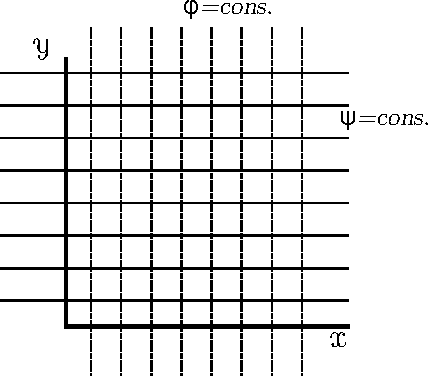
\includegraphics[width=0.5\textwidth]{clase03/flujo_uniforme.pdf}
\caption{Flujo uniforme eje x}
\label{fig:flujo_uniforme}
\end{figure}

En la Figura \ref{fig:flujo_uniforme} el flujo se mueve horizontalmente, de izquierda a derecha, con velocidad $U_\infty$.
La ecuación del potencial es $\phi=U_\infty x$, por lo que las líneas de $\phi$ constante son líneas de $x$ constante, o sea, paralelas al eje $y$.
Por otra parte, las líneas de flujo ($\psi$ constante) deben ser perpendiculares a las líneas de equipotencial.
Chequémos esto:
%
\begin{align}
\frac{\partial\psi}{\partial y} &= u = U_\infty \Rightarrow \psi=U_\infty y + f(x) \nonumber \\
\frac{\partial\psi}{\partial x} &= \frac{\partial}{\partial x}\left(U_\infty y + f(x)\right) = f'(x) = 0 \Rightarrow f(x) = C_0 = 0.
\end{align}
%
La líneas de $\psi$ constante son líneas de $y$ constante, paralelas al eje $x$, confirmando que son perpendiculares a las líneas de equipotencial.

Podemos hacer el mismo trabajo en casos parecidos.
Por ejemplo, el flujo en dirección vertical con velocidad $V_\infty$ se obtiene con $\phi=V_\infty y$, y la solución es igual a la Figura \ref{fig:flujo_uniforme}, pero con las líneas de $\phi$ y $\psi$ constante intercambiadas.
Otro caso: \mbox{?`}cómo obtener un flujo en la dirección contraria? Simplemente cambiando de signo las condiciones de borde ($-U_\infty$ o $-V_\infty$).

\subsection*{Fuente y sumidero}

\subsection*{Vórtice}

\subsection*{Doblete}
